%=========================================================================
% (c) 2011, 2012 Josef Lusticky

\chapter{Analysis}
For keeping, measuring and resolving the time, computer needs a hardware clock.
A computer clock is an electronic device with a counter register counting oscillations in a
quartz crystal oscillator with a particular frequency~\cite{thesis-sync}.
Using the hardware clock, the operating system can keep and manipulate the system time.

Accessing the hardware clock is done through the operating system clock interface.
On top of the clock interface is an interface for providing the system time.
For implementation of a reasonably useful NTP client,
the operating system must be able to set, get and eventually adjust the system time
through the time interface.
Though not mandatory, adjusting the time is an important function,
if the time shall be always a monotonically increasing function.

Apart from that, an ability to communicate over UDP is also required for the NTP client.
This is a task of the operating system network interface.
Figure~\ref{fig:analysis-overview} shows the overview of NTP client components.

\begin{figure}
  \centering
  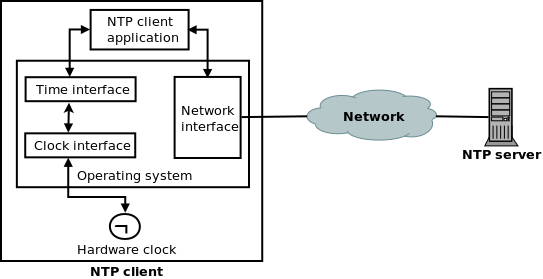
\includegraphics[width=13cm,keepaspectratio]{fig/analysis.png}
  \caption{NTP client overview} %!TODO
  \label{fig:analysis-overview} %!TODO
\end{figure}

For developing and testing Contiki NTP Client,
the AVR Raven platform with 8-bit ATmega1284P CPU~\cite{avr-datasheet} will be used.
This platform features IEEE~802.15.4 (Low-Rate Wireless Personal Area Networks) link layer support.
Together with an adaptation layer called 6LoWPAN (IPv6 over Low power Wireless Personal Area Networks),
AVR Raven is able to communicate over IPv6.

%=========================================================================
% (c) 2011, 2012 Josef Lusticky

\section{Hardware clock}\label{sec:analysis-hwclock}
On AVR Raven, Contiki uses the 8-bit Timer/Counter~2 module,
clocked from an asynchronous 32~768~Hz crystal oscillator, as the hardware clock by default.
The oscillator is independent of any other clock,
can only be used with Timer/Counter~2 and it
enables the use of Timer/Counter~2 as a Real Time Counter~\cite{avr-datasheet}.
The Timer/Counter~2 prescale value 8 is used in Contiki on the AVR Raven platform -
the oscillator frequency of 32~768~Hz is effectively divided by 8 and
the counter register is hence incremented with the frequency of
$f_{T2} = {\frac{f_{asy}}{prescaler}} = {\frac{32768}{8}} = 4096$~Hz.
Figure~\ref{fig:avr-clock} shows the Timer/Counter~2 module used by Contiki.
\begin{figure}
  \centering
  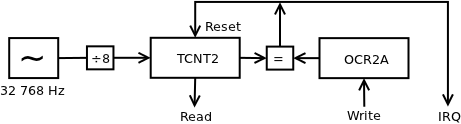
\includegraphics[width=9cm,keepaspectratio]{fig/avr-clock.png}
  \caption{Timer/Counter 2 hardware clock module on AVR Raven}
  \label{fig:avr-clock}
\end{figure}

%%Unlike I/O clock used for clocking other Timers/Counters,
%%this asynchronous crystal is also active in power-save mode~\ref{avr-datasheet}.
%CITATION: If Timer/Counter2 is enabled, it will keep running during sleep. The device can wake up from
%either Timer Overflow or Output Compare event from Timer/Counter2.
%If Timer/Counter2 is not running, Power-down mode is recommended instead of Power-save
%mode.
%The Timer/Counter2 can be clocked both synchronously and asynchronously in Power-save
%mode. If the Timer/Counter2 is not using the asynchronous clock, the Timer/Counter Oscillator is
%stopped during sleep. If the Timer/Counter2 is not using the synchronous clock, the clock source
%is stopped during sleep. Note that even if the synchronous clock is running in Power-save, this
%clock is only available for the Timer/Counter2.

The Timer/Counter~2 module is used in the Clear Timer on Compare Match (CTC) mode by Contiki.
In this mode, the counter register {\it{TCNT2}} is incrementing
and the compare register {\it{OCR2A}} defines the maximum value of the counter register.
A compare match between the counter register and the compare register
sets the Output Compare Flag {\it{OCF2A}} and resets the counter register to zero~\cite{avr-datasheet}.
This behaviour is illustrated in figure~\ref{fig:design-timing-diagram}
- the {\it{TOP}} value is equal to the value in the compare register and the {\it{BOTTOM}} value is equal to zero.

\begin{figure}
  \centering
  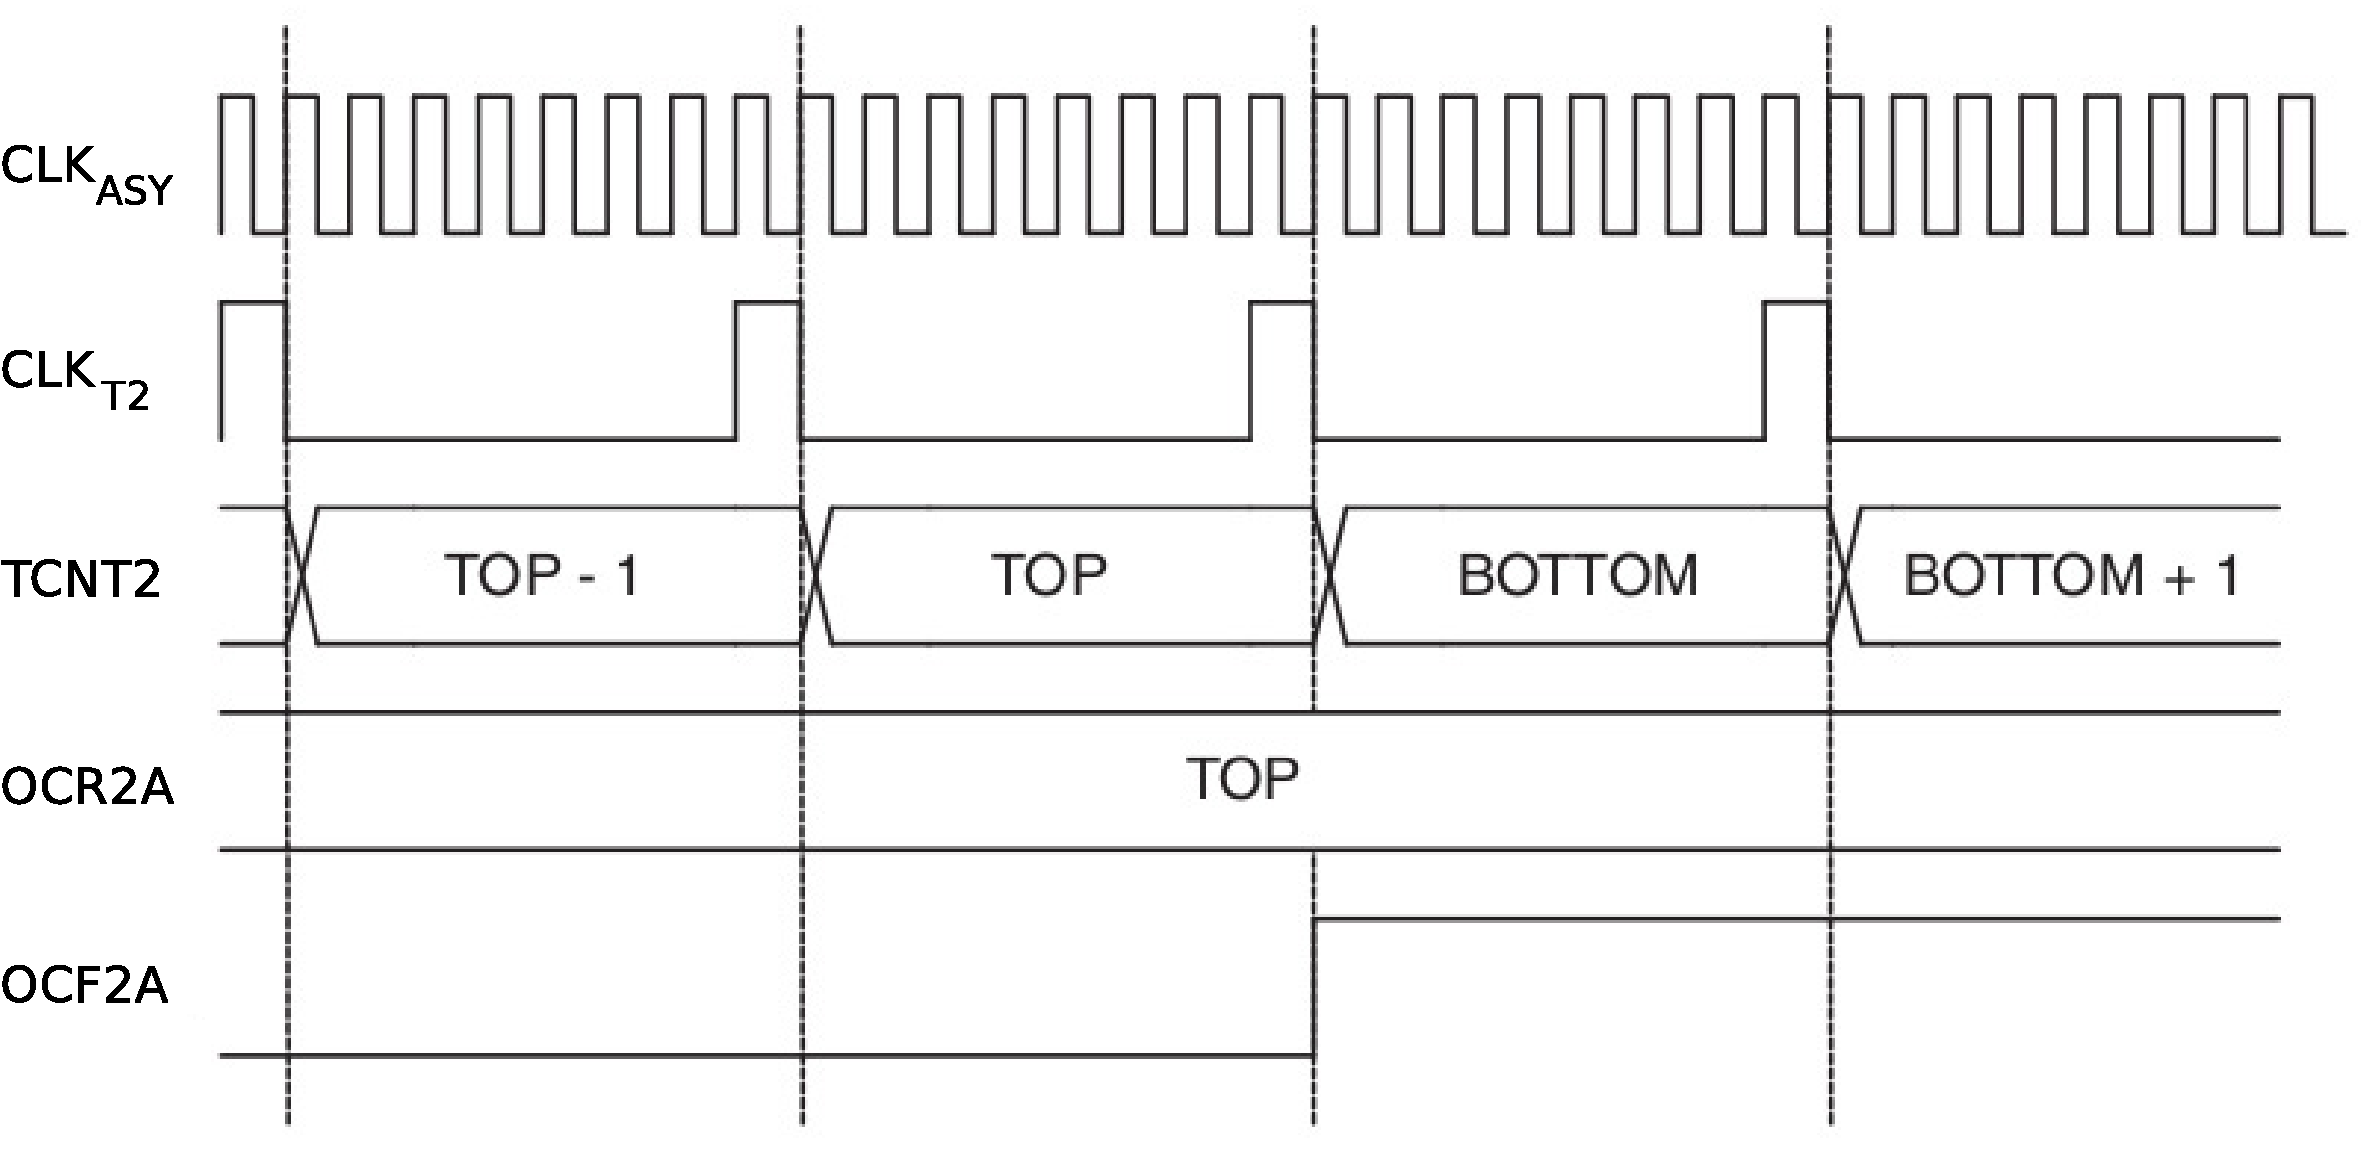
\includegraphics[width=12cm,keepaspectratio]{fig/timing-diagram.pdf}
  \caption{Timing diagram in CTC mode with prescaler 8 (source:~\cite{avr-datasheet})}
  \label{fig:design-timing-diagram}
\end{figure}

Additionally, when a compare match occurs,
an interrupt is raised and the interrupt service routine is executed.
The flag indicating occurred match {\it{OCF2A}} is
cleared automatically by hardware when executing
the interrupt service routine in this case~\cite{avr-datasheet}.

The interrupt service routine can be further used to update the value in the {\it{OCR2A}} compare register.
However, changing {\it{OCR2A}} to a value closer to zero when the counter is running
must be done with care since the CTC mode does not have a double buffering feature.
If the new value written to {\it{OCR2A}} is lower than the current
value of {\it{TCNT2}}, the counter will miss the compare match~\cite{avr-datasheet}.


%=========================================================================
% (c) 2011, 2012 Josef Lusticky

\section{Contiki clock interface}\label{sec:analysis-clock-interface}
As described in section~\ref{sec:contiki-timers},
Contiki provides a basic clock interface particularly for use of timers
with a simple goal - measuring time.
This interface is common for all supported hardware platforms,
but the particular implementation is platform-specific.
The definition of the common interface is located in the {\it{core/sys/clock.h}} file
and the specific implementations can be found in the {\it{clock.c}} file
in the {\it{cpu/}} directory of the Contiki source code.

The clock interface provides the {\it{clock\_init}} call for initialising the hardware clock,
that is automatically called during the boot sequence of Contiki.
On AVR Raven, the {\it{clock\_init}} call sets up
appropriate registers and the interrupt service routine as described in section~\ref{sec:analysis-hwclock}.

This call is implemented as a C macro and is defined in the {\it{cpu/avr/dev/clock-avr.h}} file for AVR CPUs
This macro evaluates to a specific setup code for each different AVR CPU during the compile time.
The setup code is not common to all AVR CPUs because of differences among them - e.g. there are usually
only three Timer/Counter modules, but AVR ATmega1284P has four Timer/Counter modules~\cite{avr-datasheet}.

The hardware clock interrupt, described in section~\ref{sec:analysis-hwclock},
is called {\it{clock tick}}, or {\it{timer tick}}.
At each clock tick, the interrupt service routine increments
a system clock value stored in the memory.
On AVR CPUs, there is a variable counting these clock ticks, called {\it{scount}},
and a variable counting seconds, called {\it{seconds}}.
These variables are defined together with the interrupt service routine in the {\it{cpu/avr/dev/clock.c}} file.
As described in section~\ref{sec:contiki-timers}, there are exactly {\it{CLOCK\_SECOND}} ticks in one second.
When the {\it{scount}} variable reaches the {\it{CLOCK\_SECOND}} value,
the {\it{seconds}} variable is incremented and the {\it{scount}} variable is reset.
The {\it{seconds}} variable is used by the Contiki stimers discussed in section~\ref{sec:contiki-timers}.

To obtain {\it{CLOCK\_SECOND}} interrupts per second, there must be
${\frac{f_{T2}}{CLOCK\_SECOND}}$ counter register increments between two successive interrupts.
On compare match in the CTC mode, the {\it{TCNT2}} counter register is reset to zero as
shown in figure~\ref{fig:design-timing-diagram}.
The value zero is also included in the counting - the 0th count of the timer also takes one tick.
Therefore the value of the {\it{OCR2A}} compare register must be ${\frac{f_{T2}}{CLOCK\_SECOND}} - 1$
in the CTC mode.
The default value of {\it{CLOCK\_SECOND}} for AVR Raven in Contiki is 128,
which implies the default value of the compare register ${\frac{4096}{128}} - 1 = 31$.
The {\it{CLOCK\_SECOND}} value is defined in the {\it{platform/avr-raven/contiki-conf.h}} file.
The value of the compare register is specified in the {\it{clock\_init}} call
and is computed during the compile time.


%=========================================================================
% (c) 2011, 2012 Josef Lusticky

\section{Time interface}\label{sec:analysis-time}
For keeping, measuring and resolving the time computer needs a clock.
A computer clock is an electronic device with a counter register counting oscillations in a
quartz crystal oscillator with a particular frequency~\cite{thesis-sync}.
The structure of the clock hardware is shown in figure~\ref{fig:system-hardware-clock}.
\begin{figure}
  \centering
  
\includegraphics[width=9cm,keepaspectratio]{fig/pc-clock.png}
  \caption{A typical hardware clock (source:~\cite{thesis-beat})}
  \label{fig:system-hardware-clock}
\end{figure}
When the counter reaches a specific value, an interrupt is generated and the counter register is reset.
Such interrupt is called {\it{clock tick}}, or {\it{timer tick}}, and at each clock tick,
interrupt service routine increments a system clock value stored in the memory~\cite{thesis-sync}.
In a typical computer clock design, interrupts are produced at
fixed tick intervals in the range 1-20~ms~\cite{nanokernel}.

In Contiki, such a design is used by the clock library, described in section~\ref{sec:contiki-timers}.
There is a variable counting clock ticks, called {\it{scount}},
and a variable counting seconds, called {\it{seconds}}.
As described in section~\ref{sec:contiki-timers}, there are
exactly {\it{CLOCK\_SECOND}} ticks in one second.
When the {\it{scount}} variable reaches this value,
the {\it{seconds}} variable is incremented and the {\it{scount}} variable is reset.
Both variables are used by the Contiki timers discussed in section~\ref{sec:contiki-timers}.

Since the value of the {\it{seconds}} variable is zero after the system booted,
it actually expresses the system uptime.
The {\it{seconds}} variable can be read by the application using the {\it{clock\_seconds}} call.
However, in Contiki 2.5 there is no call for setting this variable.
In the current Git version at the time of writing, a new call {\it{clock\_set\_seconds}}
can be used for this purpose.
Because this call simply rewrites the {\it{seconds}} variable, it breaks the stimer library,
and should by avoided by the NTP client.
%The {\it{clock_set_seconds}} call is implemented only for three CPU architectures at the time of writing.

The precision of one second is also not adequate for the NTP client.
Further precision can be acquired by reading the {\it{scount}} variable,
as it provides resolution of $\frac{1}{CLOCK\_SECOND}$.
Moreover, the hardware counter can be also queried, as it includes the time passed since
the last update of the {\it{scount}} variable.
If stimers should not be broken by setting the {\it{seconds}} variable,
and Contiki should be able to set and provide the current time in a higher precision,
a new call interface must be developed.

Similarly, there is no call for adjusting the time in Contiki.
Due to memory constraints, software structures controlling the time adjustments are too heavyweight
for a usage in an embedded operating system.
Due to lower CPU frequencies, the code of an interrupt service routine can not be complex
and sophisticated clock discipline algorithms should be avoided.
Because of this, a call for adjusting the time should use abilities
provided by the hardware clock as much as possible.



\section{NTP client application}
Apart from the time interface, the NTP client application needs to use the operating system network interface.
Thanks to uIP, the network communication is not a matter for Contiki OS.

The NTP client needs server associations in the NTP unicast communication mode.
However, too many server associations complicate the client design.
In fact, in the most common scenario, there can be only a single NTP master server
for the whole network.
A single server association requires just a simple calculation of the local clock offset
$\theta$, whereas more server associations require the intersection algorithm
described in section~\ref{sec:ntp-algorithms}.
Implementation of such an algorithm, requiring advanced data structures, should be avoided
in a memory constrained system.

The NTP broadcast communication mode, on the other hand,
requires no associations and no packet filling process on the client side.
Moreover, because the client does not have to actively send any NTP packets,
an energy consumption of the client is reduced.

% 1 - see design
A problem might be a possible packet loss when communication uses UDP on transport layer.
The reason why this can happen often in Contiki, is explained in section~\ref{sec:contiki-uip}.
% 2
In NTP unicast mode, the packet loss might occur either for a client's query to the server
or for a server's response to the client.
If the client's query loss occurs, no server response will be sent.
Similarly, if the server's response loss occurs, no message will be received by the client.
Not to block a whole system till the response arrives
is therefore a desired behaviour of the client.

The NTP client should be able to communicate over both IPv4 and IPv6.
Thanks to the uIP stack, this is no a matter for Contiki.
The only constraint is that both IP versions can not be used simultaneously
and the decision must be made during the compilation~\cite{contiki-docs}.
Although the {\it{UIP\_CONF\_IPV6}} macro can be used to determine which IP version
support is being compiled, the NTP client application can be written IP-version agnostic.

The NTP client further calculates the local clock offset using the NTP timestamps
as described in section~\ref{sec:ntp-algorithms}.
As mentioned in section~\ref{sec:ntp-time}, the NTP timescale is not
coincident with the POSIX timescale.
If the new calls in the time interface should use the standard POSIX timescale,
conversion between NTP and POSIX timestamps must be calculated.
The conversion from the POSIX timestamp to the 64-bit long NTP timestamp
is needed when the client sends the request
and the conversion vice versa is needed when the client calculates
the local clock offset from the received timestamps.

Since both timescales reckon in seconds, the conversion between
the NTP timestamp seconds field value and the POSIX timestamp seconds field value is simple.
However, the conversion between the NTP fraction field value ($2^{-32}$)
and the POSIX fraction field value (nanoseconds or microseconds) is problematic.
The relation between the POSIX fraction field and the NTP fraction field
is given by $POSIX.frac = NTP.frac \times POSIX.res \div 2^{32}$,
where $POSIX.frac$ is the POSIX fraction field value,
$NTP.frac$ is the NTP fraction field value and
$POSIX.res$ is the POSIX timestamp resolution (microseconds or nanoseconds).
The accurate conversion requires either floating point operations or operations with 64 bit numbers.
These operations can be memory expensive, especially on 8-bit microcontrollers,
and their usage must be considered carefully or another suitable solution must be found.
